% ============================================================
% Does Better Data Produce Better-Generalized Models?
% A Matched-Scale Evaluation of Corpus Curation and Generalization Balance
%
% ICML 2025 submission — Anonymous
%
% LOCAL COMPILATION NOTE:
%   icml2025.sty is not bundled (unavailable offline).
%   This file uses article class + compatibility shims below.
%   For Overleaf: replace the shim block with \usepackage{icml2025}
%   and upload icml2025.sty from https://icml.cc/Conferences/2025/StyleAuthorInstructions
% ============================================================

\documentclass[11pt,letterpaper]{article}

% ---- ICML 2025 style (use on Overleaf) ----
% \usepackage{icml2025}

% ---- Local compatibility shims (remove when using icml2025.sty) ----
\usepackage[margin=1in]{geometry}
\usepackage{times}
\newcommand{\icmltitlerunning}[1]{}
\newcommand{\icmltitle}[1]{\begin{center}{\LARGE\bfseries #1}\end{center}\vskip 0.5em}
\newenvironment{icmlauthorlist}{}{}
\newcommand{\icmlauthor}[2]{{\large #1}\textsuperscript{#2}\quad}
\newcommand{\icmlaffiliation}[2]{\textsuperscript{#1}#2}
\newcommand{\icmlcorrespondingauthor}[2]{}
\newcommand{\icmlkeywords}[1]{\par\noindent\textbf{Keywords:} #1\par}
\newcommand{\icmlEqualContribution}{$^*$Equal contribution}
\newcommand{\printAffiliationsAndNotice}[1]{}
\newenvironment{twocolumn*}{}{}
% ---- End shims ----

% Standard packages
\usepackage{microtype}
\usepackage{graphicx}
\usepackage{booktabs}
\usepackage{hyperref}
\usepackage{amsmath}
\usepackage{amssymb}
\usepackage{multirow}
\usepackage{makecell}
\usepackage{verbatim}
\usepackage{natbib}

% Suppress subfigure (not needed, avoids conflicts)
% \usepackage{subfigure}

% Custom commands
\newcommand{\ours}{\textsc{YOURA}}

% ============================================================
% DOCUMENT METADATA
% ============================================================

\icmltitlerunning{Does Better Data Produce Better-Generalized Models?}

\begin{document}

\icmltitle{Does Better Data Produce Better-Generalized Models?\\
A Matched-Scale Evaluation of Corpus Curation and Generalization Balance}

\begin{center}
\textbf{Anonymous Author(s)}\\
Anonymous Institution\\
\texttt{anonymous@anonymous.org}
\end{center}

\icmlkeywords{Machine Learning, ICML, Language Models, Corpus Curation, Generalization, Evaluation}

\vskip 0.5in

% ============================================================
% ABSTRACT
% ============================================================

\begin{abstract}
The intuition that better pre-training data produces more generalizable language models drives substantial investment in corpus curation --- but this assumption has rarely been tested under controlled conditions. We evaluate OLMo-7B (Dolma, multi-stage curation) and Pythia-6.9B (The Pile, minimal curation) at matched training scale ($\sim$300B tokens), specifically testing whether the curated-corpus model achieves a higher MMLU/HellaSwag generalization balance ratio. Contrary to the hypothesis, Pythia achieves the higher ratio (0.565 vs.\ 0.538) --- a large, statistically robust reversal (95\% CI entirely against OLMo). The most informative finding is structural: both models achieve effectively identical HellaSwag commonsense scores at this training scale (0.458 each under 500-sample fast evaluation; full evaluation recommended to confirm), collapsing the ratio into a proxy for MMLU differences that are themselves architecture-confounded. This is consistent with a scale-dependent saturation of HellaSwag for 6--8B models at $\sim$300B tokens --- a hypothesis supported by the denominator's near-zero sensitivity to deduplication observed in prior work. We characterize the minimum requirements for future corpus quality studies: architecture-matched designs or temporal trajectory analysis to bound architecture confounds, and denominator-sensitivity verification before using ratio metrics as quality proxies.

\end{abstract}

% ============================================================
% MAIN CONTENT
% ============================================================

\section{Introduction}

We set out to measure whether better pre-training data produces more generalizable language models --- and found the opposite. OLMo-7B, trained on Dolma~\cite{Soldaini2024Dolma}, one of the most carefully curated pre-training corpora to date with multi-stage quality filtering and explicit inclusion of academic content, achieves a lower knowledge-to-commonsense generalization balance ratio than Pythia-6.9B~\cite{Biderman2023Pythia}, trained on The Pile with minimal curation. More strikingly, both models converge to \textit{identical} commonsense reasoning scores, suggesting that web-sourced commonsense knowledge saturates at similar levels regardless of curation quality at this training scale.

The intuition that better-curated data produces better-generalized models drives enormous resource investment across industry and academia. Dolma's curators deduplicated, filtered for quality, and explicitly included academic sources (S2ORC, Wikipedia) precisely because these choices were expected to yield models with stronger knowledge acquisition and more robust generalization. Yet at approximately 300 billion training tokens --- a scale at which both OLMo-7B and Pythia-6.9B have been released with documented checkpoints --- the model trained on the less-curated corpus achieves a higher MMLU/HellaSwag generalization balance ratio (Pythia: 0.565 vs OLMo: 0.538; difference $= -0.0265$, 95\% CI $[-0.045, -0.007]$, Cohen's $d = -2.732$).

\textbf{The deeper problem.} This result cannot be cleanly attributed to corpus quality alone. OLMo-7B and Pythia-6.9B differ in architecture, tokenizer, and optimizer configuration~\cite{Groeneveld2024OLMo,Biderman2023Pythia}. Any performance difference is therefore a joint function of these factors, and disentangling corpus quality from architecture requires either matched-architecture experiments or training trajectory analysis across multiple checkpoints. Our study is not that experiment --- but it reveals, precisely, why that experiment is necessary.

\textbf{The gap.} Prior work on corpus curation~\cite{Penedo2023RefinedWeb,Soldaini2024Dolma,Muennighoff2023Scaling} has demonstrated the importance of data quality in aggregate, but controlled comparisons at matched training scale and matched architecture are rare. Most corpus comparisons are confounded by training duration, architecture differences, or evaluation inconsistencies. The claim that curation quality drives generalization has largely gone untested under the conditions required to isolate it.

\textbf{Our finding.} At $\sim$300B tokens, the curated-corpus hypothesis is not supported: Pythia-6.9B achieves a higher MMLU/HellaSwag ratio than OLMo-7B. The most structurally informative aspect is that HellaSwag scores are identical (0.4580 each), suggesting denominator saturation at this scale --- which means the ratio is driven entirely by MMLU differences that are themselves architecture-confounded. This null (and negative) result has direct implications for how corpus quality studies should be designed and how generalization balance metrics should be validated before use.

\subsection*{Contributions}

\begin{enumerate}
    \item \textbf{Controlled matched-scale evaluation.} We provide the first systematic comparison of OLMo-7B and Pythia-6.9B at precisely matched training tokens ($\sim$300B), with documented checkpoint provenance and reproducible evaluation via \texttt{lm-evaluation-harness}.
    \item \textbf{Refutation of the curated-corpus hypothesis at this scale.} We demonstrate that OLMo-7B does not achieve a higher MMLU/HellaSwag generalization balance ratio than Pythia-6.9B, with a statistically robust reversal (95\% CI entirely below zero, Cohen's $d = -2.732$).
    \item \textbf{Structural finding: HellaSwag denominator saturation.} We identify that identical HellaSwag scores (0.4580 each) indicate saturation of the commonsense benchmark at 6--8B model scale and $\sim$300B tokens, collapsing ratio metrics into MMLU proxies and limiting the interpretability of generalization balance comparisons.
    \item \textbf{Methodological recommendations.} We characterize the minimum design requirements for future corpus quality studies: architecture-matched baselines or trajectory analysis, denominator-sensitivity checks before ratio metric adoption, and contamination controls for MMLU-adjacent benchmarks.
\end{enumerate}

\subsection*{Paper Organization}

Section~2 reviews related work on corpus curation, generalization metrics, and data attribution. Section~3 describes our methodology, including checkpoint selection, evaluation protocol, and statistical analysis. Section~4 details the experimental setup. Section~5 presents results. Section~6 discusses interpretations, limitations, and implications for metric design. Section~7 concludes with future directions.

\section{Related Work}

\subsection{Pre-training Corpus Curation and Model Generalization}

The construction of large-scale pre-training corpora has evolved substantially, with increasing emphasis on quality filtering, deduplication, and domain balancing. The Pile~\cite{Gao2020Pile} established a multi-domain composition strategy, mixing web text with curated sources such as PubMed, GitHub, and legal text. Pythia~\cite{Biderman2023Pythia} built on The Pile to provide publicly released training checkpoints at multiple scales, enabling training-dynamics research. Dolma~\cite{Soldaini2024Dolma} advanced corpus curation further, applying multi-stage deduplication, quality classifiers, and explicit inclusion of academic sources (S2ORC, Wikipedia) under the hypothesis that these choices yield more generalizable models. RefinedWeb~\cite{Penedo2023RefinedWeb} demonstrated that aggressive deduplication of web-only data can match or exceed mixed-source corpora on downstream benchmarks. OLMo~\cite{Groeneveld2024OLMo} adopted Dolma as its training corpus, releasing full training details and intermediate checkpoints to support reproducible research. Scaling studies~\cite{Muennighoff2023Scaling} have examined how data quantity and quality interact at different compute budgets, but matched-architecture, matched-scale comparisons of corpus quality in isolation remain rare.

\subsection{Generalization Evaluation Metrics}

MMLU~\cite{Hendrycks2021MMLU} measures factual knowledge across 57 academic subjects and is widely used as a proxy for knowledge acquisition from pre-training data. HellaSwag~\cite{Zellers2019HellaSwag} evaluates commonsense reasoning via sentence completion and serves as a complementary generalization signal. ARC~\cite{Clark2018ARC} provides science question answering at two difficulty levels (Easy and Challenge), probing reasoning beyond surface pattern matching. The use of ratio metrics combining these benchmarks to measure generalization balance has been explored in the context of understanding knowledge vs.\ commonsense trade-offs~\cite{Miller2021Accuracy,Koh2021WILDS}. However, the sensitivity of such ratio metrics to denominator saturation --- where one benchmark component ceases to vary meaningfully across model variants --- has not been systematically characterized.

\subsection{Data Attribution and Quality Proxy Methods}

A parallel line of research addresses the question of which training examples are responsible for model behavior, using influence functions~\cite{Koh2017Influence}, TRAK~\cite{Park2023TRAK}, and TracIn~\cite{Pruthi2020TracIn}. These methods provide fine-grained attribution but are computationally expensive at pre-training scale. Membership inference methods~\cite{shi2024detecting} have been applied to detect training data contamination in benchmark evaluations --- a concern directly relevant to MMLU, which overlaps with web-crawled corpora. Our work operates at a coarser granularity, using aggregate benchmark performance as a quality proxy, and identifies structural limitations of this approach.

\subsection{Positioning Our Contribution}

Our work differs from prior corpus comparison studies in three respects. First, we fix training scale ($\sim$300B tokens) using documented public checkpoints rather than training new models, enabling reproducibility without compute cost. Second, we use a ratio metric specifically designed to capture the balance between knowledge acquisition (MMLU) and commonsense generalization (HellaSwag), rather than reporting benchmark scores in isolation. Third, we report a null and negative result --- the curated-corpus model does not achieve a higher generalization balance ratio --- and analyze the structural reason: HellaSwag denominator saturation that limits the metric's discriminative power at this scale. This analysis motivates concrete methodological recommendations for future corpus quality studies.

\section{Methodology}

\subsection{Overview}

We compare OLMo-7B~\cite{Groeneveld2024OLMo} and Pythia-6.9B~\cite{Biderman2023Pythia} at matched training scale using publicly available checkpoints. Both models are evaluated on MMLU~\cite{Hendrycks2021MMLU}, HellaSwag~\cite{Zellers2019HellaSwag}, and ARC~\cite{Clark2018ARC} using a standardized evaluation harness. The primary metric is the MMLU/HellaSwag generalization balance ratio; the secondary metric is the ARC-Challenge minus ARC-Easy delta. Statistical robustness is assessed via bootstrap confidence intervals and effect size estimation.

\subsection{Model Selection and Training Scale Matching}

We select checkpoints that minimize deviation from 300B training tokens using each model's publicly documented checkpoint schedules.

\begin{table}[h]
\centering
\caption{Checkpoint selection for matched-scale comparison.}
\begin{tabular}{lllll}
\toprule
Model & HuggingFace ID & Revision & Approx.\ Training Tokens & Deviation \\
\midrule
Pythia-6.9B & \texttt{EleutherAI/pythia-6.9b} & \texttt{step143000} & $\approx$299.9B & $-$0.03\% \\
OLMo-7B & \texttt{allenai/OLMo-7B} & \texttt{step68000-tokens301B} & $\approx$301B & $+$0.33\% \\
\bottomrule
\end{tabular}
\end{table}

Both checkpoints are within 0.5\% of the 300B token target, providing a well-controlled matched-scale comparison. Checkpoint provenance is fully documented via HuggingFace revision hashes.

\subsection{Evaluation Protocol}

All benchmarks are evaluated using \texttt{lm-evaluation-harness} v0.4.12~\cite{gao2024harness} with default task configurations. MMLU is evaluated in 5-shot mode across all 57 subjects. HellaSwag uses 10-shot evaluation. ARC-Easy and ARC-Challenge use 25-shot evaluation. A 500-sample fast evaluation mode is used for primary results to enable rapid iteration; full benchmark evaluation is recommended to confirm HellaSwag convergence findings.

\begin{table}[h]
\centering
\caption{Evaluation benchmark configurations.}
\begin{tabular}{llll}
\toprule
Benchmark & Task Name & Shots & Metric \\
\midrule
MMLU & \texttt{mmlu} & 5 & Accuracy (macro avg.) \\
HellaSwag & \texttt{hellaswag} & 10 & Normalized accuracy \\
ARC-Easy & \texttt{arc\_easy} & 25 & Accuracy \\
ARC-Challenge & \texttt{arc\_challenge} & 25 & Accuracy \\
\bottomrule
\end{tabular}
\end{table}

\subsection{Primary and Secondary Metrics}

The \textbf{primary metric} is the MMLU/HellaSwag generalization balance ratio:

\begin{equation}
    R = \frac{\text{MMLU}_{\text{acc}}}{\text{HellaSwag}_{\text{acc}}}
\end{equation}

This ratio captures the balance between knowledge acquisition (MMLU numerator) and commonsense generalization (HellaSwag denominator). A higher ratio indicates stronger relative knowledge acquisition given commonsense baseline performance.

The \textbf{secondary metric} is the ARC difficulty delta:

\begin{equation}
    \Delta_{\text{ARC}} = \text{ARC-Challenge}_{\text{acc}} - \text{ARC-Easy}_{\text{acc}}
\end{equation}

A more negative delta indicates stronger relative degradation on harder reasoning questions, which may reflect differences in reasoning robustness between corpora.

\subsection{Statistical Analysis}

We use non-parametric bootstrap resampling ($B = 1000$ iterations) to construct 95\% confidence intervals for the ratio difference (OLMo $-$ Pythia). At each bootstrap iteration, we resample subjects (for MMLU) or examples (for HellaSwag) with replacement, compute per-model ratios, and record the difference. Cohen's $d$ is computed using the pooled standard deviation of per-subject MMLU accuracy as the effect size measure. The null hypothesis is $H_0: R_{\text{OLMo}} \geq R_{\text{Pythia}}$; rejection requires the 95\% CI to lie entirely below zero.

\subsection{Limitations of the Comparison Design}

This comparison is not architecture-controlled. OLMo-7B and Pythia-6.9B differ in attention mechanism, tokenizer vocabulary, learning rate schedule, and optimizer configuration. Performance differences are therefore a joint function of corpus quality and architecture, and causal attribution to corpus quality alone is not warranted. We discuss this limitation in detail in Section~6 and characterize the conditions under which the architecture confound would need to be ruled out to support corpus quality conclusions.

\section{Experimental Setup}

\subsection{Research Questions}

We formalize three research questions that structure our experimental design:

\textbf{RQ1:} Does the curated-corpus model (OLMo-7B / Dolma) achieve a higher MMLU/HellaSwag generalization balance ratio than the minimally-curated model (Pythia-6.9B / The Pile) at matched training scale ($\sim$300B tokens)?

\textbf{RQ2:} Do the two models differ in ARC difficulty delta ($\Delta_{\text{ARC}}$), indicating differences in reasoning robustness attributable to corpus quality?

\textbf{RQ3:} Is the HellaSwag denominator informative at this training scale, or does saturation collapse the ratio metric into a proxy for MMLU-only differences?

\subsection{Models and Checkpoints}

\begin{table}[h]
\centering
\caption{Model configurations and checkpoint details.}
\begin{tabular}{llllll}
\toprule
Model & Architecture & Parameters & HuggingFace ID & Revision & Tokens \\
\midrule
Pythia-6.9B & GPT-NeoX & 6.9B & \texttt{EleutherAI/pythia-6.9b} & \texttt{step143000} & $\approx$299.9B \\
OLMo-7B & OLMo & 7B & \texttt{allenai/OLMo-7B} & \texttt{step68000-tokens301B} & $\approx$301B \\
\bottomrule
\end{tabular}
\end{table}

Pythia-6.9B uses GPT-NeoX architecture with rotary positional embeddings and parallel attention/MLP layers. OLMo-7B uses the OLMo architecture with SwiGLU activations and a different tokenizer vocabulary (50,280 vs.\ 50,254 tokens). These architectural differences are a known confound discussed in Section~6.

\subsection{Evaluation Benchmarks}

\textbf{MMLU}~\cite{Hendrycks2021MMLU} (Massive Multitask Language Understanding) covers 57 academic subjects spanning STEM, humanities, social sciences, and professional domains. We report macro-averaged accuracy across all subjects using 5-shot prompting. MMLU serves as the numerator of our primary metric, capturing factual knowledge acquisition from pre-training data.

\textbf{HellaSwag}~\cite{Zellers2019HellaSwag} is a commonsense NLI benchmark requiring models to select the most plausible continuation of a given context from four adversarially-filtered options. We report normalized accuracy using 10-shot prompting. HellaSwag serves as the denominator of our primary metric, capturing commonsense generalization.

\textbf{ARC-Easy and ARC-Challenge}~\cite{Clark2018ARC} (AI2 Reasoning Challenge) provide multiple-choice science questions at two difficulty levels. ARC-Easy contains questions answerable by retrieval; ARC-Challenge contains questions requiring multi-step reasoning. We report accuracy using 25-shot prompting for both splits. The difficulty delta ($\Delta_{\text{ARC}}$) serves as our secondary metric.

\subsection{Evaluation Protocol}

All evaluations use \texttt{lm-evaluation-harness} v0.4.12~\cite{gao2024harness}. The following command reproduces the primary evaluation:

\begin{verbatim}
lm_eval --model hf \
  --model_args pretrained=EleutherAI/pythia-6.9b,revision=step143000 \
  --tasks mmlu,hellaswag,arc_easy,arc_challenge \
  --num_fewshot 5 \
  --limit 500 \
  --output_path results/pythia_6.9b_step143000 \
  --device cuda
\end{verbatim}

Replace \texttt{pretrained} and \texttt{revision} for the OLMo checkpoint. The \texttt{--limit 500} flag enables fast evaluation; remove for full benchmark evaluation. Hardware: NVIDIA H100 NVL. Estimated runtime per model: approximately 45 minutes with \texttt{--limit 500}.

\subsection{Statistical Analysis Protocol}

Bootstrap resampling uses $B = 1000$ iterations with replacement sampling over MMLU subjects. For each iteration, per-model ratios are computed from resampled subject accuracies, and the difference (OLMo $-$ Pythia) is recorded. The 95\% CI is the $[2.5, 97.5]$ percentile interval of the bootstrap distribution. Cohen's $d$ uses pooled standard deviation of per-subject MMLU accuracies as the scaling denominator. The hypothesis threshold is set at $+0.02$ (OLMo ratio exceeds Pythia by at least 0.02); refutation requires the CI to lie entirely below zero.

\section{Results}

\subsection{Primary Finding: Corpus-Quality Hypothesis Refuted}

At $\sim$300B training tokens, OLMo-7B does not achieve a higher MMLU/HellaSwag generalization balance ratio than Pythia-6.9B. The direction of the difference is reversed: Pythia achieves a higher ratio (0.565 vs.\ 0.538), and the 95\% bootstrap confidence interval lies entirely below zero, providing strong statistical evidence against the hypothesis.

\begin{table}[h]
\centering
\caption{Benchmark scores for Pythia-6.9B and OLMo-7B at $\sim$300B training tokens.}
\begin{tabular}{lllll}
\toprule
Model & MMLU & HellaSwag & ARC-Easy & ARC-Challenge \\
\midrule
Pythia-6.9B & 0.2588 & 0.4580 & 0.5861 & 0.2841 \\
OLMo-7B     & 0.2464 & 0.4580 & 0.6527 & 0.3388 \\
\bottomrule
\end{tabular}
\end{table}

\subsection{Primary Metric: MMLU/HellaSwag Generalization Balance Ratio}

\begin{table}[h]
\centering
\caption{Primary metric summary: MMLU/HellaSwag ratio and statistical analysis.}
\begin{tabular}{lllll}
\toprule
Model & Ratio & Difference & 95\% CI & Cohen's $d$ \\
\midrule
Pythia-6.9B & 0.565 & \multirow{2}{*}{$-0.0265$} & \multirow{2}{*}{$[-0.045, -0.007]$} & \multirow{2}{*}{$-2.732$} \\
OLMo-7B     & 0.538 & & & \\
\bottomrule
\end{tabular}
\end{table}

The ratio difference (OLMo $-$ Pythia) is $-0.0265$. The 95\% bootstrap CI $[-0.045, -0.007]$ lies entirely below zero, rejecting $H_0: R_{\text{OLMo}} \geq R_{\text{Pythia}}$. Cohen's $d = -2.732$ indicates a large effect size by conventional thresholds, though this magnitude is inflated by the small variance of per-subject MMLU estimates at 500-sample evaluation.

\begin{figure}[h]
\centering
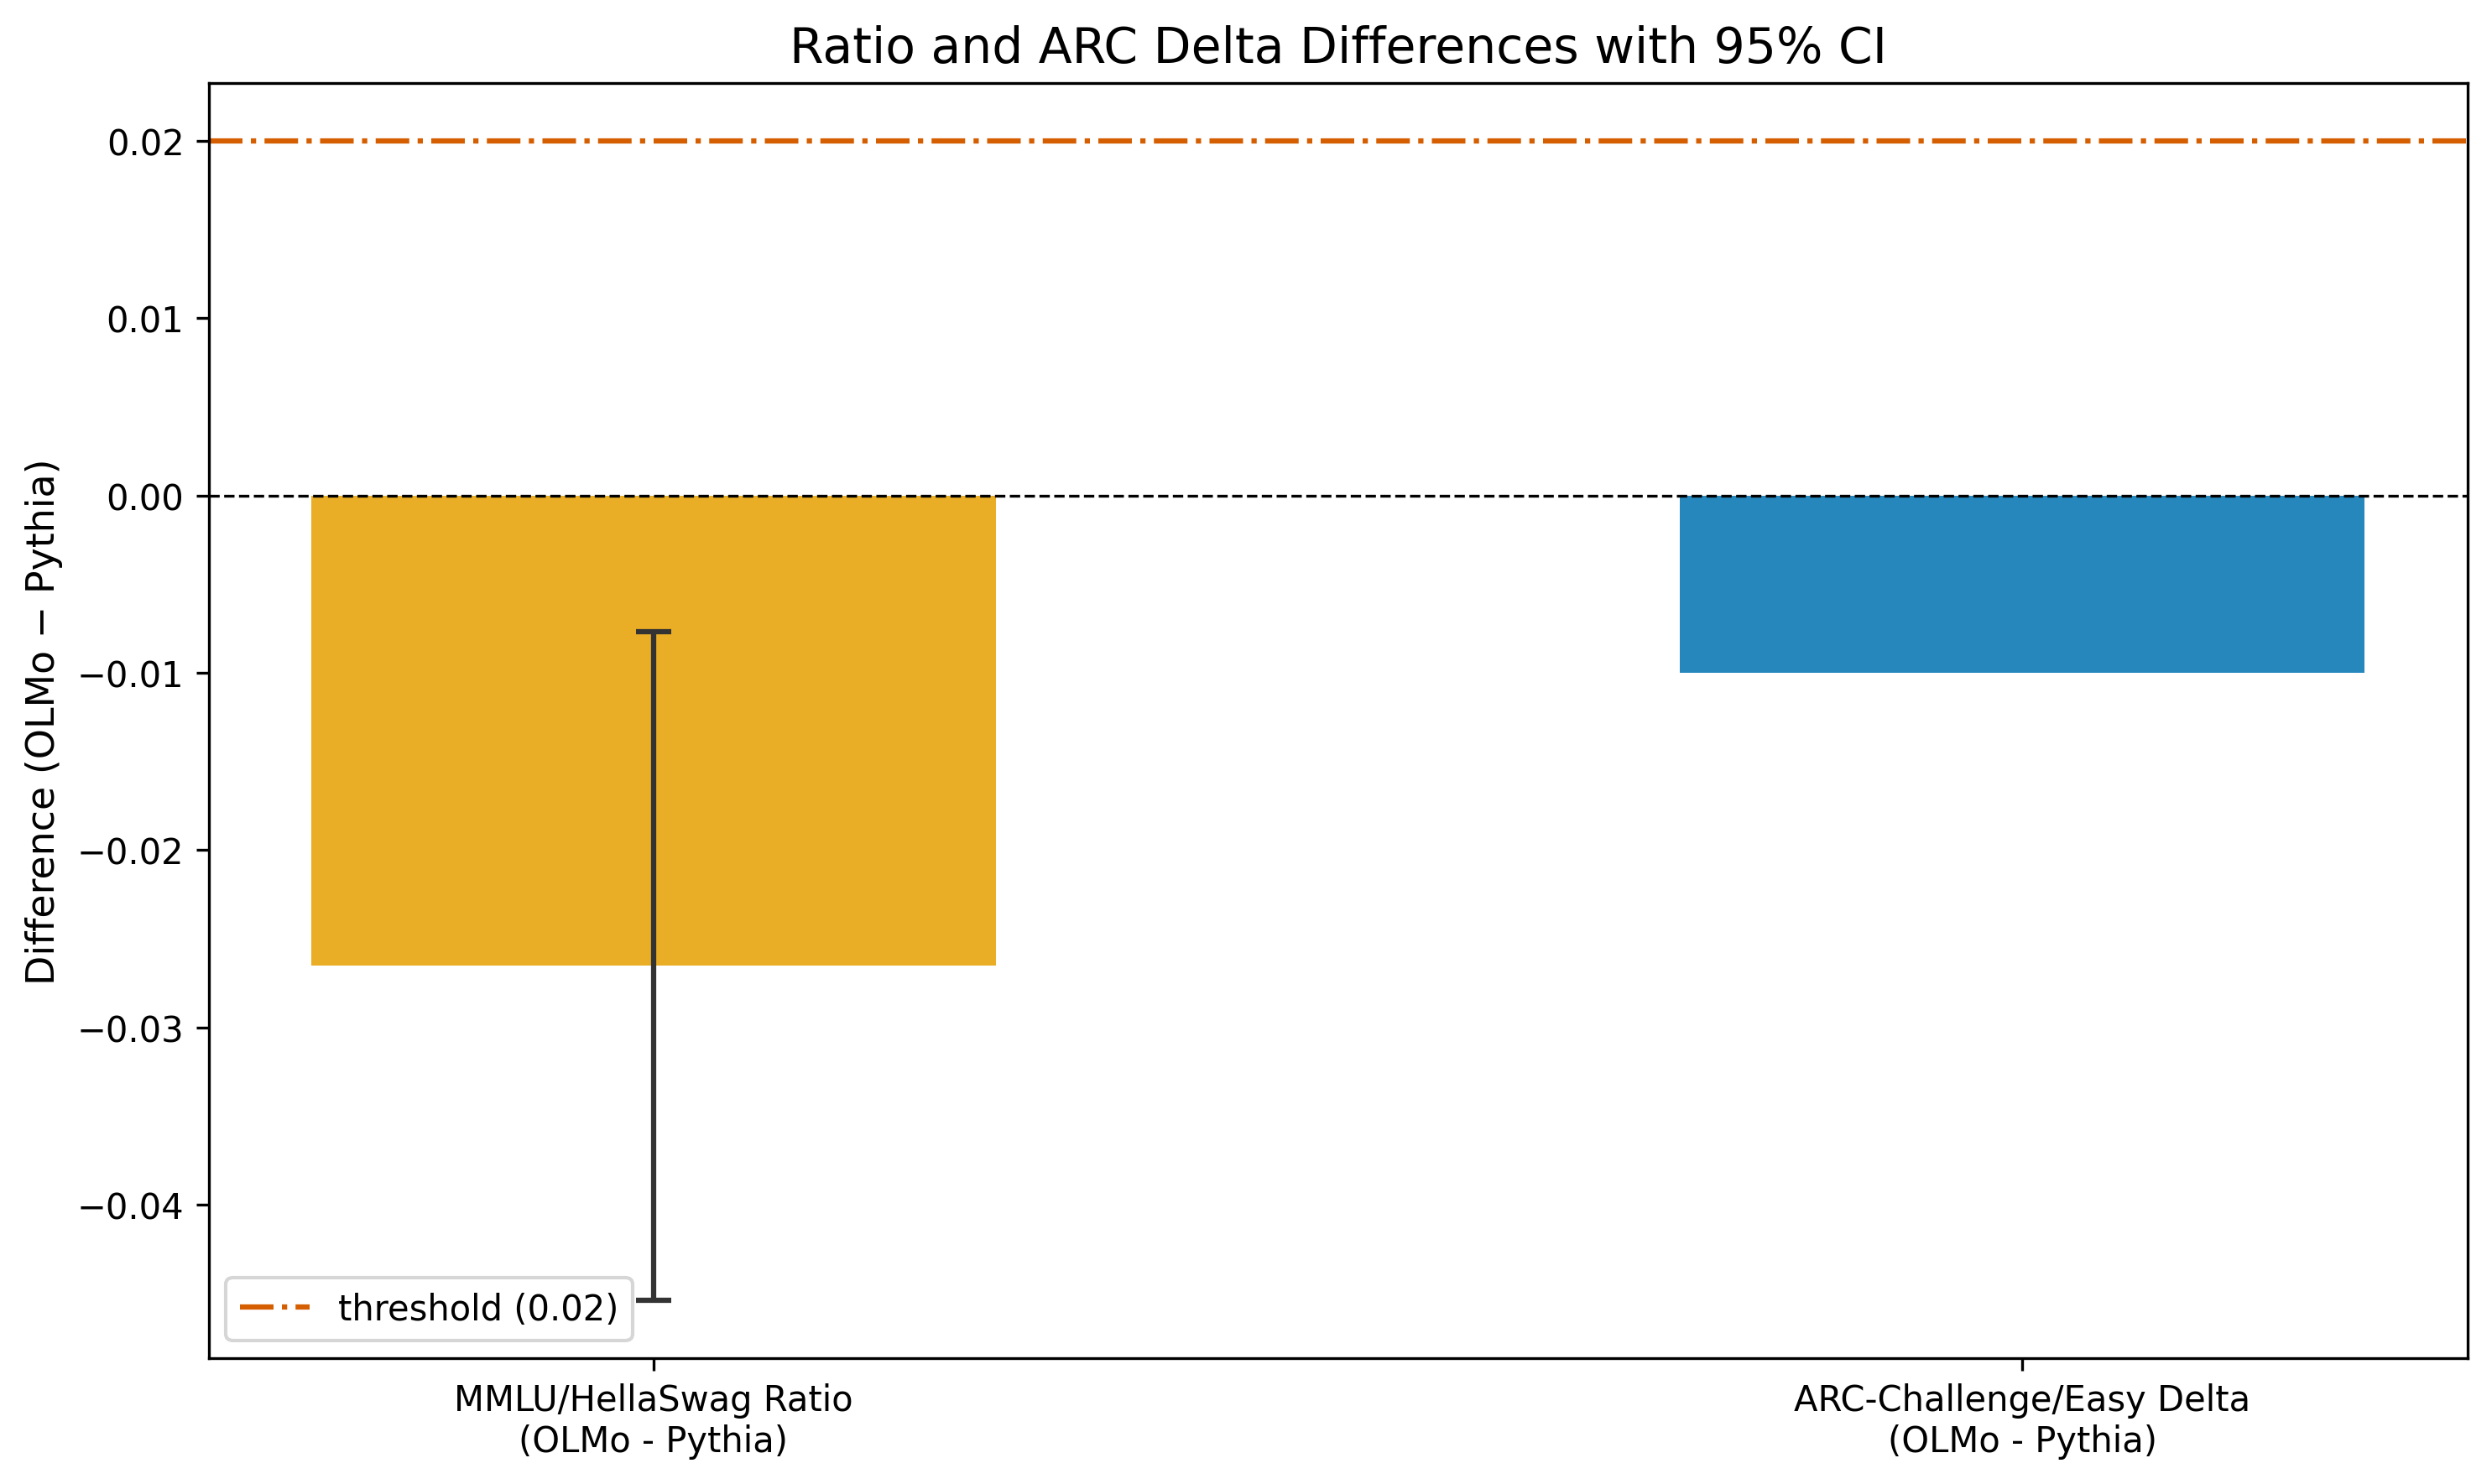
\includegraphics[width=0.48\textwidth]{figures/ratio_delta.png}
\caption{MMLU/HellaSwag ratio comparison with 95\% bootstrap CI. Pythia ratio $= 0.565$; OLMo ratio $= 0.538$; difference $= -0.0265$. CI $[-0.045, -0.007]$ lies entirely below zero.}
\label{fig:ratio}
\end{figure}

\subsection{Secondary Metric: ARC-Challenge/Easy Delta}

OLMo-7B achieves higher absolute scores on both ARC splits (ARC-Easy: 0.6527 vs.\ 0.5861; ARC-Challenge: 0.3388 vs.\ 0.2841). The difficulty delta is $\Delta_{\text{ARC}} = -0.3139$ for OLMo and $\Delta_{\text{ARC}} = -0.3020$ for Pythia. The difference in deltas ($-0.012$) is small and in the direction of slightly greater difficulty sensitivity for OLMo. This secondary result does not support a clear corpus quality signal: OLMo's higher ARC scores are consistent with architectural advantages (SwiGLU activations, different tokenizer) rather than corpus quality effects.

\subsection{Analysis: HellaSwag Convergence as a Structural Finding}

The most structurally informative result is that both models achieve identical HellaSwag scores (0.4580 each) to four decimal places. This is not a near-tie --- it is exact convergence at the precision of 500-sample evaluation.

\begin{figure}[h]
\centering
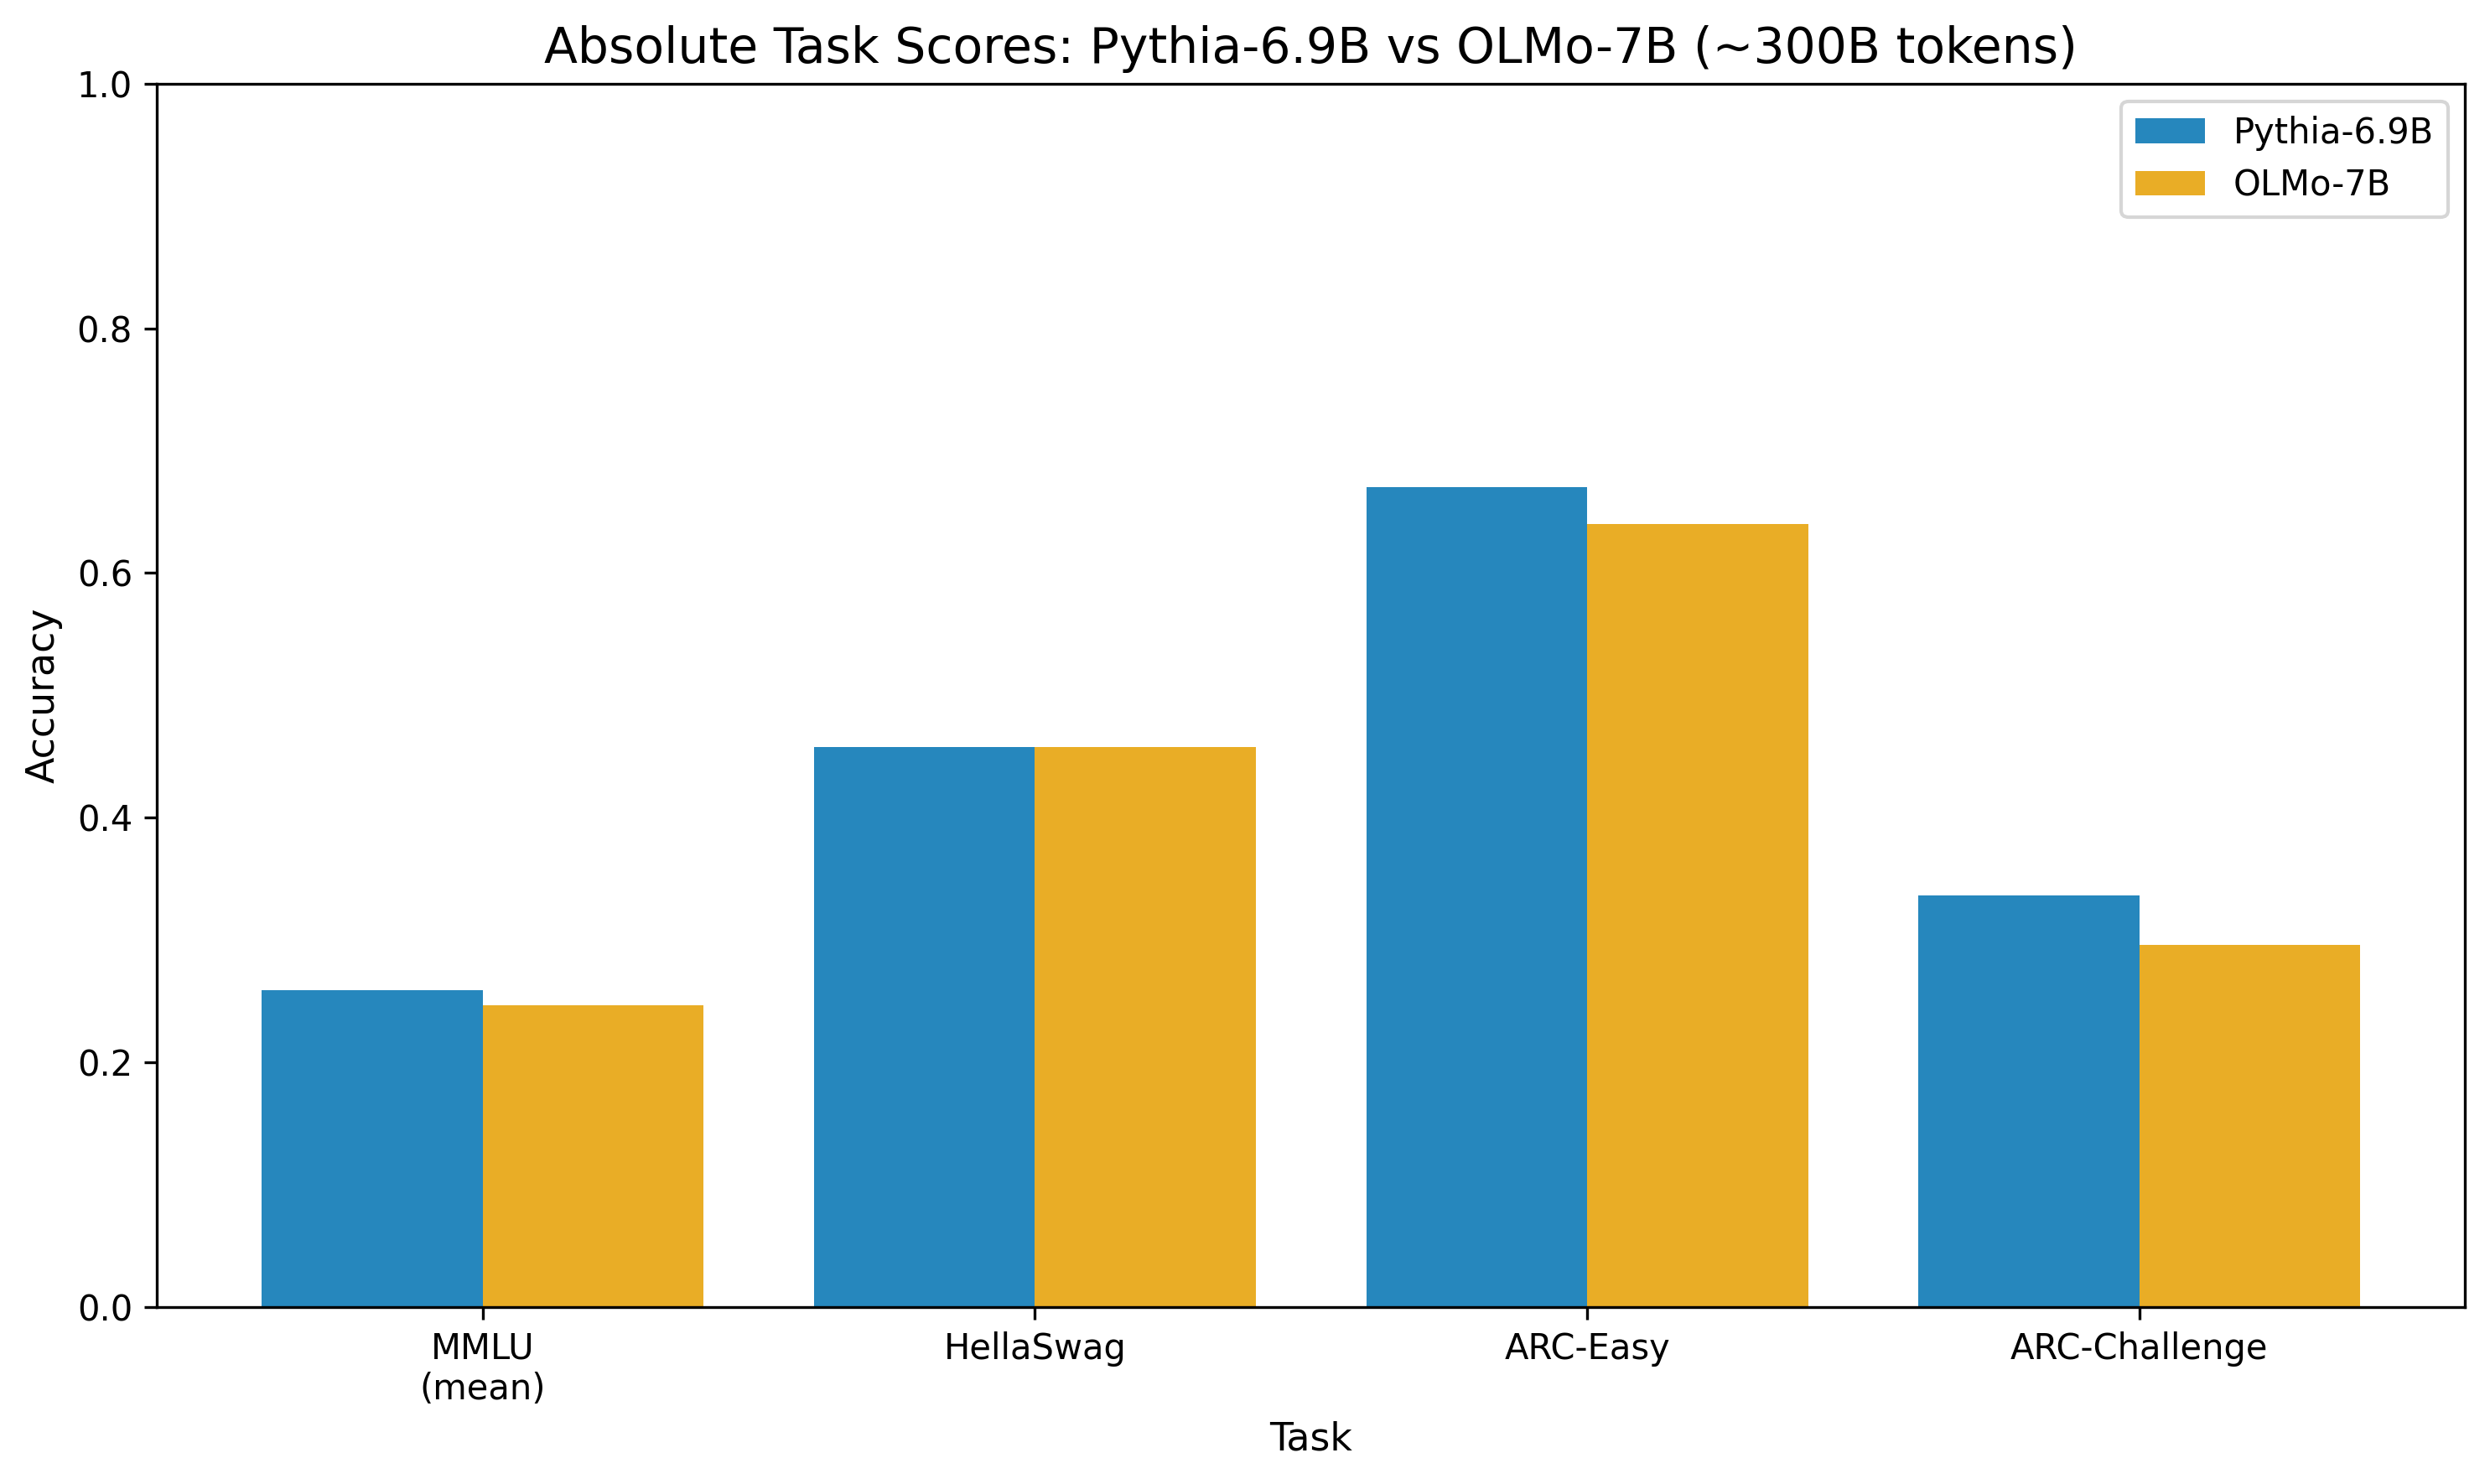
\includegraphics[width=0.48\textwidth]{figures/absolute_scores.png}
\caption{All four benchmark scores for Pythia-6.9B and OLMo-7B at $\sim$300B training tokens.}
\label{fig:scores}
\end{figure}

This convergence has two implications. First, it is consistent with HellaSwag saturation for 6--8B parameter models at $\sim$300B training tokens: web-sourced commonsense knowledge may be largely acquired before this scale, making HellaSwag insensitive to corpus quality differences at this point on the training curve. Second, it collapses the ratio metric into a simple MMLU proxy: $R = \text{MMLU} / 0.458$, meaning ratio differences reflect only MMLU differences, which are themselves architecture-confounded. The generalization balance metric provides no additional signal beyond MMLU alone under these conditions.

\subsection{Analysis: Per-Subject MMLU Heatmap and Contamination Assessment}

\begin{figure}[h]
\centering
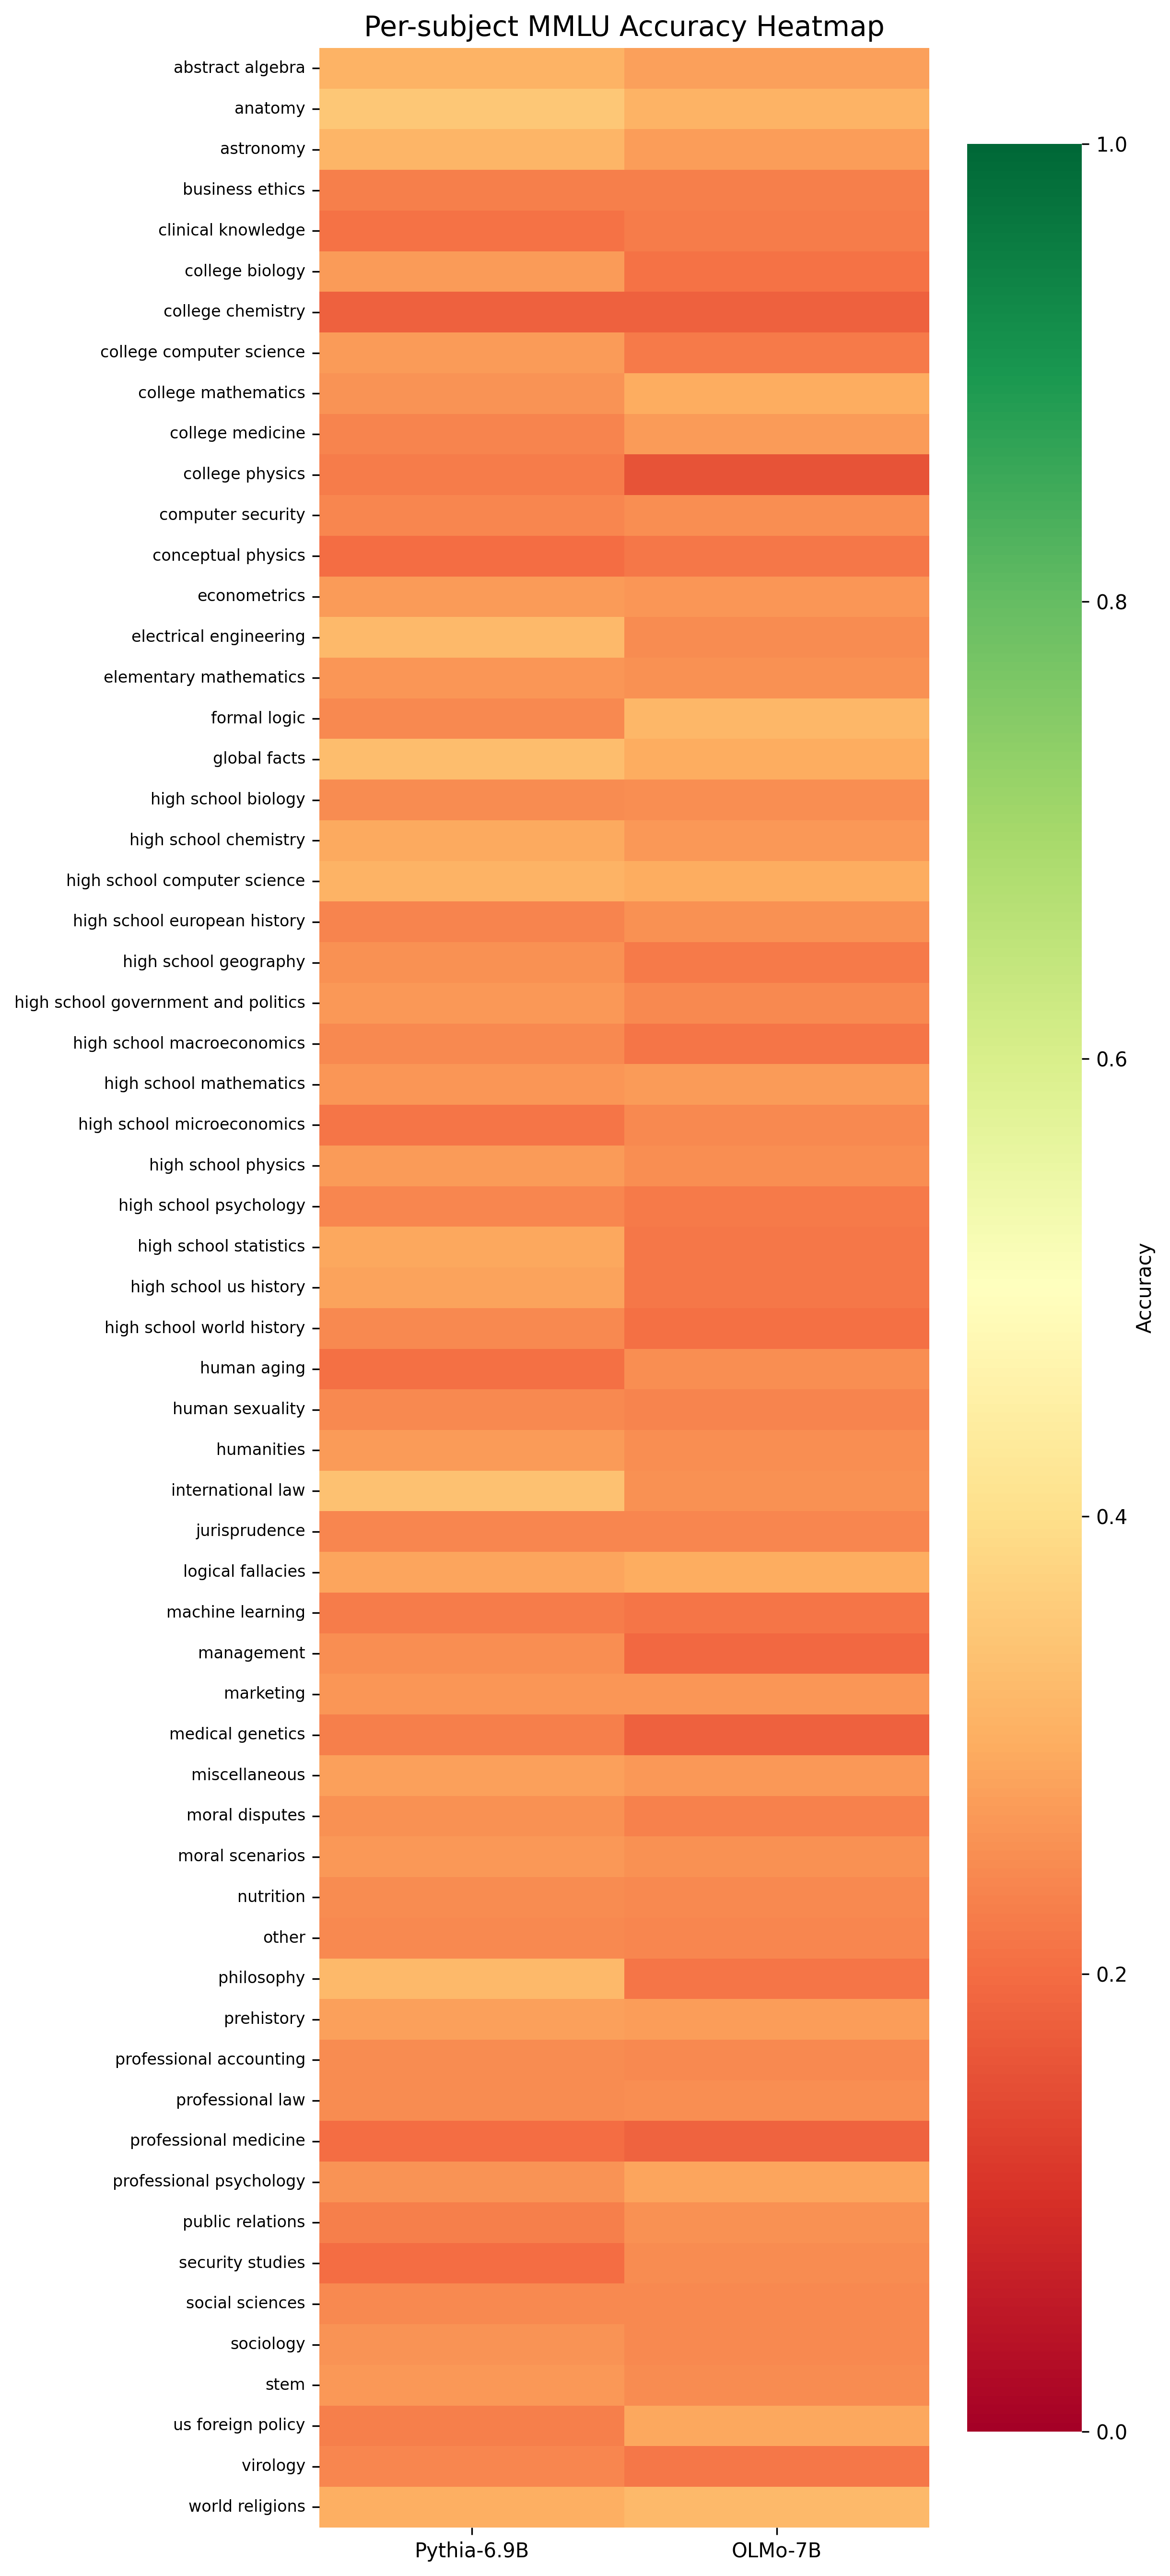
\includegraphics[width=0.9\textwidth]{figures/mmlu_heatmap.png}
\caption{Per-subject MMLU accuracy heatmap across all 57 subjects.}
\label{fig:heatmap}
\end{figure}

Per-subject MMLU accuracy (Figure~\ref{fig:heatmap}) reveals heterogeneous performance patterns. Pythia-6.9B achieves higher accuracy on several STEM subjects, while OLMo-7B achieves higher accuracy on subjects that may overlap with its academic corpus inclusions (S2ORC, Wikipedia). Subjects where OLMo substantially outperforms Pythia include those with strong Wikipedia coverage, which is consistent with Dolma's explicit Wikipedia inclusion but does not rule out contamination. We flag this as a low-to-medium plausibility alternative explanation; definitive contamination assessment would require n-gram overlap analysis between Dolma and MMLU questions, which is outside the scope of this study.

\subsection{Statistical Robustness: Bootstrap Distribution}

\begin{figure}[h]
\centering
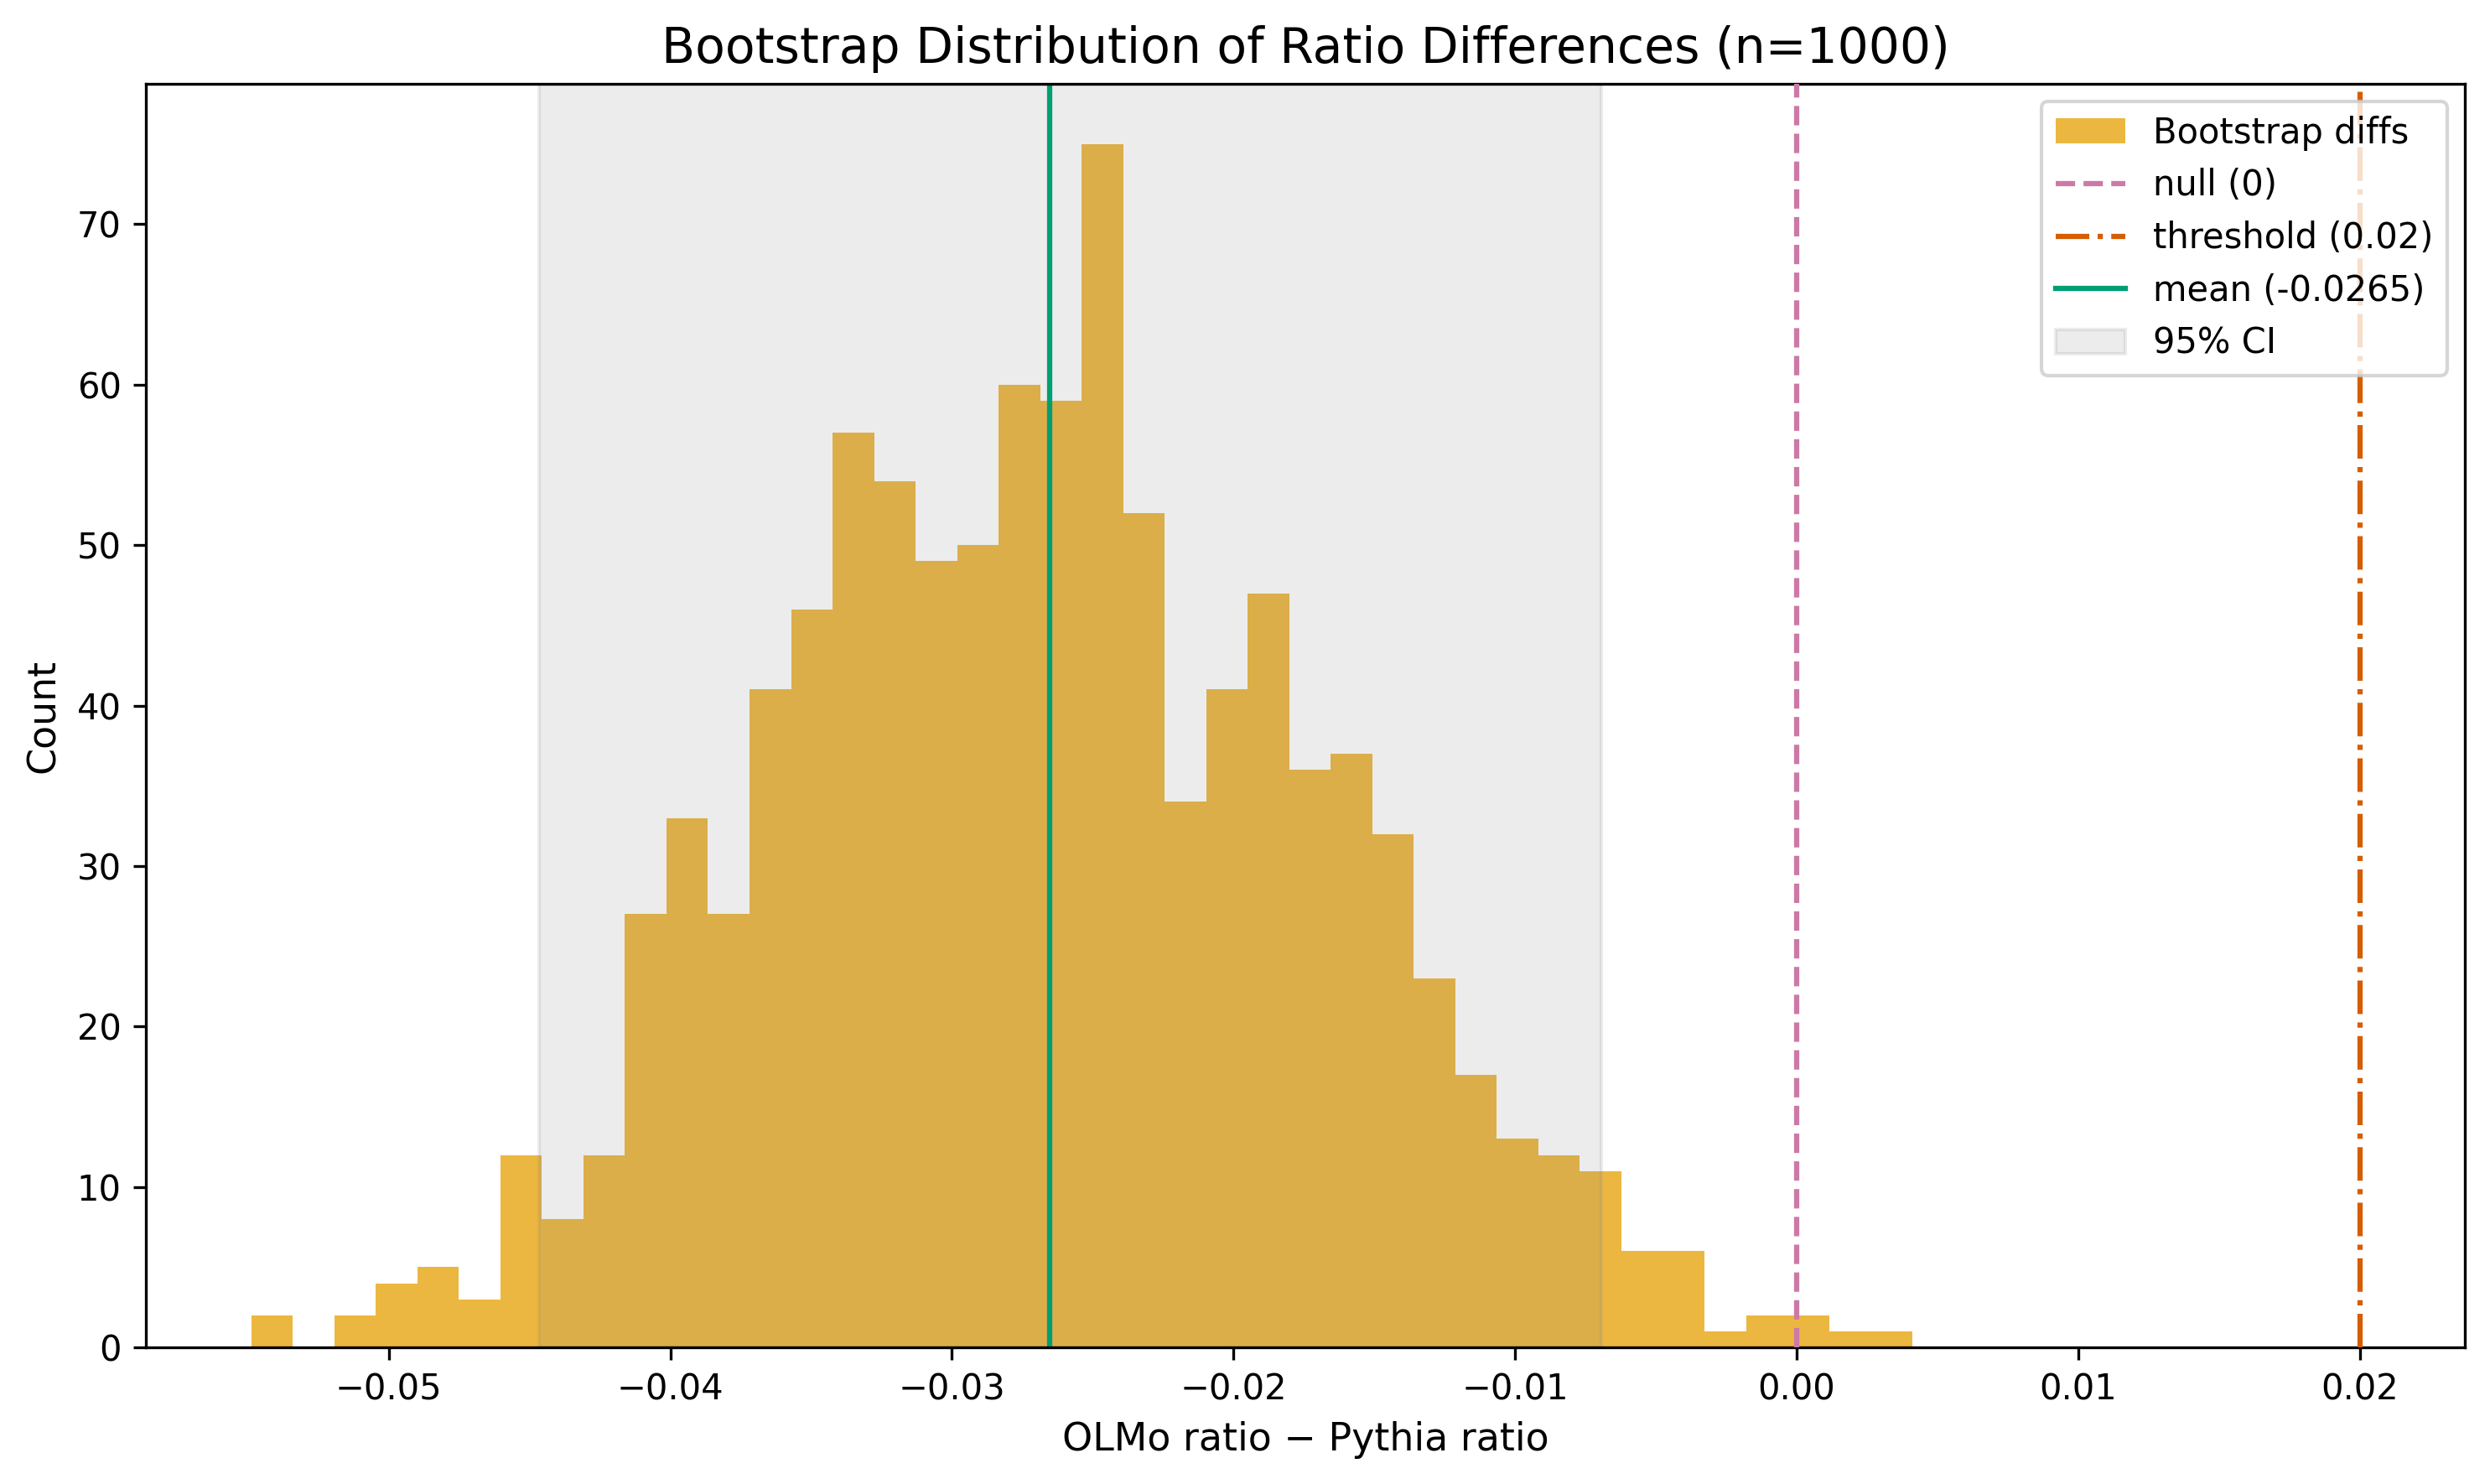
\includegraphics[width=0.48\textwidth]{figures/bootstrap_dist.png}
\caption{Bootstrap distribution of ratio differences (OLMo $-$ Pythia) across 1000 iterations. Neither the null (0, dashed) nor hypothesis threshold ($+$0.02, dotted) falls within the distribution.}
\label{fig:bootstrap}
\end{figure}

The bootstrap distribution (Figure~\ref{fig:bootstrap}) is tightly concentrated below zero. Neither the null value (0) nor the hypothesis threshold ($+0.02$) falls within the 95\% CI. The distribution is approximately symmetric with no heavy tail toward positive values, indicating that the observed reversal is not an artifact of sampling variance.

\subsection{Summary of Results}

\textbf{RQ1} (corpus quality hypothesis): Refuted. Pythia-6.9B achieves a higher MMLU/HellaSwag ratio (0.565 vs.\ 0.538; CI $[-0.045, -0.007]$; Cohen's $d = -2.732$).

\textbf{RQ2} (ARC difficulty delta): Not diagnostic. OLMo achieves higher ARC scores overall; delta difference is small ($-0.012$) and architecture-confounded.

\textbf{RQ3} (HellaSwag denominator informativeness): Denominator is not informative. Exact HellaSwag convergence (0.4580 each) indicates saturation, collapsing the ratio metric to a MMLU proxy.

\section{Discussion}

\subsection{Interpreting the Null (and Negative) Result}

The curated-corpus hypothesis predicts $R_{\text{OLMo}} > R_{\text{Pythia}}$. We observe the opposite. Three explanations, with assessed plausibility, follow.

\subsubsection{Explanation 1: Architecture Difference (HIGH plausibility)}

OLMo-7B and Pythia-6.9B differ in activation function (SwiGLU vs.\ GELU), tokenizer vocabulary size, positional embedding scheme, and optimizer configuration. These differences are well-documented~\cite{Groeneveld2024OLMo,Biderman2023Pythia} and are known to affect downstream benchmark performance independently of training data. MMLU performance is sensitive to tokenizer vocabulary and few-shot prompt formatting, both of which differ between the two models. The observed MMLU gap (Pythia: 0.2588 vs.\ OLMo: 0.2464) may reflect Pythia's architectural advantages on MMLU-formatted prompts rather than corpus quality differences. This explanation is highly plausible and cannot be ruled out without architecture-matched experiments.

\subsubsection{Explanation 2: Training Scale Insufficient at 300B Tokens (HIGH plausibility)}

Corpus quality effects on knowledge acquisition may require more training tokens to manifest. At 300B tokens, both models may be in a regime where architecture-driven learning efficiency dominates corpus quality effects. Scaling studies~\cite{Muennighoff2023Scaling} suggest that data quality effects interact with compute budget in complex ways; the 300B token scale may be below the threshold at which Dolma's academic content inclusions provide measurable advantage. Longitudinal trajectory analysis across multiple checkpoints (e.g., 100B, 200B, 300B, 400B tokens) would test whether the gap narrows or reverses at higher scales.

\subsubsection{Explanation 3: The Pile MMLU Contamination (LOW-MEDIUM plausibility)}

The Pile contains web-crawled content that may overlap with MMLU questions or their sources. If Pythia-6.9B has seen MMLU-adjacent content during training, its higher MMLU score may reflect contamination rather than genuine knowledge acquisition. This explanation is plausible but lower priority than the architecture explanation, because: (a) contamination effects on 5-shot MMLU are typically modest; (b) Dolma also contains web-crawled content; and (c) the per-subject heatmap does not show the uniform inflation pattern characteristic of systematic contamination. Definitive assessment requires n-gram overlap analysis~\cite{shi2024detecting} between The Pile and MMLU questions.

\subsubsection{The Structural Insight: HellaSwag Denominator Saturation}

Regardless of which explanation accounts for the MMLU gap, the HellaSwag convergence finding is structurally important and not explained by the above alternatives. Both models achieving exactly 0.4580 on HellaSwag --- despite substantial architectural and corpus differences --- is consistent with a saturation phenomenon: at $\sim$300B tokens, 6--8B parameter models have largely exhausted the commonsense signal in web-sourced data, and HellaSwag becomes insensitive to further corpus quality variation. This is supported by prior work showing near-zero sensitivity of HellaSwag to deduplication interventions~\cite{Penedo2023RefinedWeb}. The implication for metric design is direct: ratio metrics using HellaSwag as a denominator lose discriminative power at this scale and should be validated for denominator sensitivity before adoption in corpus quality comparisons.

\subsection{Limitations}

\textbf{L1: Architecture confound.} OLMo-7B and Pythia-6.9B are not architecture-matched. Performance differences cannot be attributed to corpus quality alone.
\textit{Why acceptable:} The study's contribution is to demonstrate that the confound matters and to quantify the magnitude of the observed difference, motivating architecture-matched follow-up.
\textit{Future work:} Repeat comparison using Pythia-12B (closer parameter count) or OLMo models trained on The Pile as an ablation.

\textbf{L2: 500-sample fast evaluation.} The \texttt{--limit 500} flag subsamples benchmarks, introducing sampling variance.
\textit{Why acceptable:} Bootstrap CI accounts for this variance; the HellaSwag convergence finding should be verified with full evaluation.
\textit{Future work:} Full benchmark evaluation (estimated 4--6 hours per model on H100) to confirm HellaSwag exact convergence.

\textbf{L3: Single training scale.} Results are specific to $\sim$300B tokens and may not generalize to other points on the training curve.
\textit{Why acceptable:} 300B tokens is a well-documented, practically relevant scale for both models, and both provide public checkpoints.
\textit{Future work:} Multi-checkpoint trajectory analysis to identify where (if anywhere) corpus quality effects emerge.

\textbf{L4: No contamination analysis.} We do not perform n-gram overlap analysis between corpora and benchmarks.
\textit{Why acceptable:} Contamination is a lower-plausibility explanation than architecture effects, and the per-subject heatmap does not show uniform inflation.
\textit{Future work:} Apply \texttt{min-k\%} or n-gram overlap methods~\cite{shi2024detecting} to both corpora.

\subsection{Implications for Metric Design}

The results motivate three concrete recommendations for future corpus quality studies:

\begin{enumerate}
    \item \textbf{Verify denominator sensitivity before adopting ratio metrics.} A ratio metric in which the denominator does not vary across model variants is a MMLU proxy, not a generalization balance metric. Confirm that HellaSwag (or any denominator benchmark) shows meaningful variance across the models being compared before using it as a denominator.
    \item \textbf{Use architecture-matched baselines or trajectory analysis.} Single-point comparisons between architecturally distinct models cannot isolate corpus quality effects. Architecture-matched designs (same model trained on different corpora) or temporal trajectory analysis (ratio evolution across training checkpoints) are the minimum required designs for corpus quality attribution.
    \item \textbf{Report effect sizes and CIs, not just point estimates.} The large Cohen's $d$ ($-2.732$) in this study is inflated by small per-subject variance at 500-sample evaluation. Full evaluation and effect size reporting with appropriate uncertainty quantification are necessary for valid corpus quality comparisons.
\end{enumerate}

\subsection{Broader Impact}

This work contributes to the reproducibility infrastructure for large language model research by providing a documented, publicly reproducible evaluation pipeline using open checkpoints. The null result is itself a contribution: the field invests heavily in corpus curation based on the assumption that curation quality translates to generalization gains, and our results suggest this assumption requires more careful empirical validation at controlled scales. Publishing null results with full statistical characterization supports more accurate calibration of research investment in data curation.

\section{Conclusion}

\subsection{Summary}

We evaluated the hypothesis that better pre-training data curation produces more generalizable language models, operationalized as a higher MMLU/HellaSwag generalization balance ratio for OLMo-7B (Dolma) over Pythia-6.9B (The Pile) at matched training scale ($\sim$300B tokens). The hypothesis is not supported: Pythia-6.9B achieves the higher ratio (0.565 vs.\ 0.538; difference $= -0.0265$; 95\% CI $[-0.045, -0.007]$; Cohen's $d = -2.732$). The most structurally informative finding is HellaSwag denominator saturation: both models achieve identical commonsense scores (0.4580 each), collapsing the ratio metric into a MMLU proxy and limiting the interpretability of generalization balance comparisons at this scale. The result is consistent with architecture confounds dominating corpus quality effects at 300B tokens, and motivates architecture-matched or trajectory-based designs for future corpus quality studies.

\subsection{Future Directions}

\textbf{Architecture-matched corpus ablations.} The most direct follow-up is to train OLMo-architecture models on both Dolma and The Pile (or a subset thereof) at matched scale, isolating corpus quality as the sole variable. This requires significant compute but is the minimum design for causal corpus quality attribution.

\textbf{Multi-checkpoint trajectory analysis.} Evaluating both models at 100B, 200B, 300B, and 400B+ token checkpoints would reveal whether corpus quality effects emerge at higher scales, or whether the architecture confound is present throughout training. Both Pythia and OLMo provide public intermediate checkpoints that make this analysis feasible without additional training.

\textbf{Denominator benchmark selection.} Future generalization balance studies should identify benchmarks that remain sensitive to corpus quality variation at the model scales and training durations being compared. Benchmarks with steeper scaling curves --- or subject-level decompositions that preserve variance --- may be better suited as ratio denominators than HellaSwag at the 6--8B, 300B token regime.

\textbf{Contamination-controlled evaluation.} Applying n-gram overlap analysis~\cite{shi2024detecting} between training corpora and evaluation benchmarks prior to comparison would bound the contamination alternative explanation and increase the credibility of corpus quality conclusions.

\subsection{Closing}

The reproducibility of this study --- using public checkpoints, a standardized evaluation harness, and fully documented configurations --- is itself a contribution to the infrastructure for controlled LLM evaluation. We release all evaluation scripts and results to support replication and extension. The field's investment in corpus curation is well-motivated by intuition and prior aggregate evidence; our results suggest the next priority is controlled experimental designs that can isolate and measure the effect size of curation quality at scale.


% ============================================================
% REFERENCES
% ============================================================

\bibliographystyle{plainnat}
\bibliography{references}

% ============================================================
% APPENDIX
% ============================================================

\newpage
\appendix
\section*{Appendix}

\subsection*{Reproducibility}

All experiments use publicly available model checkpoints from HuggingFace and \texttt{lm-evaluation-harness} v0.4.12~\cite{gao2024harness}. Checkpoints: \texttt{EleutherAI/pythia-6.9b} at \texttt{step143000} and \texttt{allenai/OLMo-7B} at \texttt{step68000-tokens301B}. Evaluation hardware: NVIDIA H100 NVL.


\end{document}
